\documentclass{beamer}

\usepackage[spanish, mexico]{babel}
\usepackage{amsmath}
\usepackage{amsfonts}
\usepackage{amssymb}
\usepackage[utf8]{inputenc}

\usetheme{Warsaw}

\title{Función Binomial Negativa}
\author{Glenn R., Miguel G.}
\institute{Fundación Universitaria Konrad Lorenz}
\date{28-09-2019}

\begin{document}
    \maketitle
    \begin{frame}
		\frametitle{Función Binomial Negativa}
		\framesubtitle{Introducción}
		En teoría de la probabilidad y estadística, una distribución binomial negativa es una distribución de probabilidad discreta del número de éxitos en una secuencia independiente e idéntica de intentos de Bernoulli\footnote{O intentos binomiales, es decir, en un experimento sólo pueden ocurrir dos cosas éxito o fallo.} antes de que un número de fallos (no aleatorios) ocurran.
		\begin{figure}
			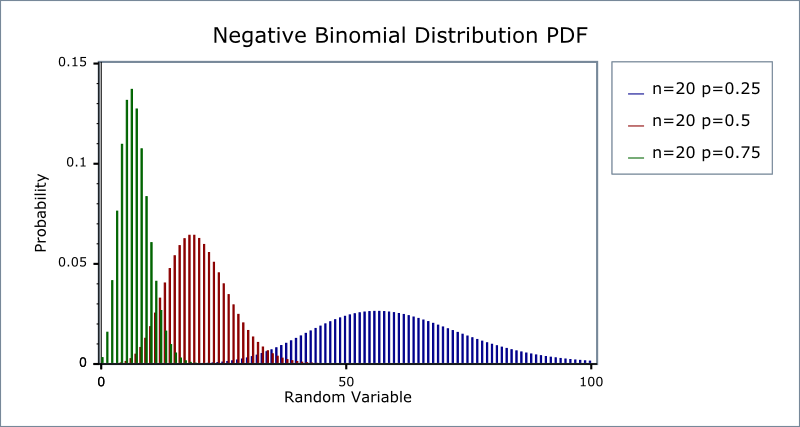
\includegraphics[width=0.6\linewidth]{negative-bimonial.png}
			\caption{PDF: Probability Distribution Function.}
			\label{fig:andrew}
		\end{figure}
	\end{frame}
	\begin{frame}
		\frametitle{Función Binomial Negativa}
		\framesubtitle{Definición}
		Suponga que existe una secuencia de intentos independientes de Bernoulli. Para cada intento existen dos potenciales resultados llamados \textit{éxito} y \textit{fallo}. En cada intento la probabilidad de éxito es $p$ y la probabilidad de fallo es $(1 - p)$. Observamos esta secuencia hasta un número predefinido de que $r$ fallos hayan ocurrido. Entonces, el número aleatorio de éxitos que evidenciamos, $X$, tendrá el negativo binomial de la distribución, es decir:
		
        $${X\sim \operatorname {NB} (r,p)}$$
	\end{frame}
	\begin{frame}
		\frametitle{Función Binomial Negativa}
		\framesubtitle{Formulas: Función de probabilidad}
		$$f(x) = P(X = x) = \binom{x - 1}{r - 1} p^r (1 - p)^{x-r}$$
		Donde:
		\begin{itemize}
		    \item $X$ es el intento en el cual el r-ésimo éxito ocurre.
		    \item $r \geq 1, r \in \mathbb{N}$
		    \item $0 < p \leq 1, p \in \mathbb{Q}$
		    \item $x = r, r + 1, r + 2, r + 3, \dots , r + q, q \in \mathbb{N}$
		\end{itemize}
	\end{frame}
	\begin{frame}
		\frametitle{Función Binomial Negativa}
		\framesubtitle{Formulas: Media}
		$$\mu = E(X) = \frac{r}{p}$$
		Donde:
		\begin{itemize}
		    \item $X$ es el intento en el cual el r-ésimo éxito ocurre.
		    \item $r \geq 1, r \in \mathbb{N}$
		    \item $0 < p \leq 1, p \in \mathbb{Q}$
		\end{itemize}
	\end{frame}
	\begin{frame}
		\frametitle{Función Binomial Negativa}
		\framesubtitle{Formulas: Varianza}
		$$\sigma = Var(X) = \frac{r(1-p)}{p^2}$$
		Donde:
		\begin{itemize}
		    \item $X$ es el intento en el cual el r-ésimo éxito ocurre.
		    \item $r \geq 1, r \in \mathbb{N}$
		    \item $0 < p \leq 1, p \in \mathbb{Q}$
		\end{itemize}
	\end{frame}
	\begin{frame}
		\frametitle{Función Binomial Negativa}
		\framesubtitle{¿Porqué es importante? (Aplicación)}
		Para predecir si el resultado de un proyecto será el adecuado, si la probabilidad de que ocurran muchos fracasos es alta lo mas viable y sensato sería descartar su ejecución para no incurrir en costos innecesarios.
	\end{frame}
	\begin{frame}{Ejemplo I}
	    \begin{examples}
            Se sabe que la probabilidad de que un niño expuesto a una enfermedad contagiosa la contraiga es de 0.4. Obtener la probabilidad de que el décimo niño estudiado sea el tercero en contraer la enfermedad.
        \end{examples}
	\end{frame}
	\begin{frame}{Ejemplo II}
	    \begin{examples}
            En un proceso de manufactura se sabe que un promedio de 1 en cada 10 productos es defectuoso, ¿cual es la probabilidad que el quinto (5) artículo examinado sea el primero (1) en estar defectuoso?
        \end{examples}
	\end{frame}
	\begin{frame}{Ejemplo II: solución}
	    \begin{figure}
    		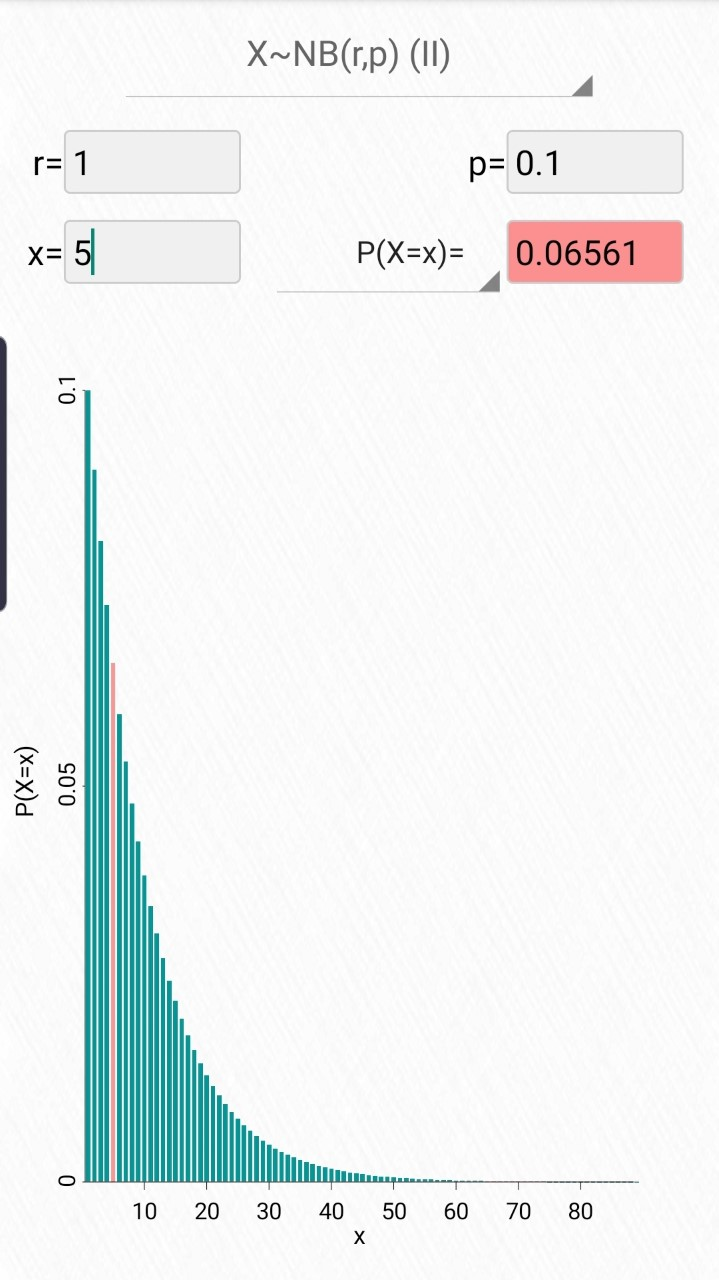
\includegraphics[width=0.4\linewidth]{II.jpg}
		\end{figure}
	\end{frame}
	\begin{frame}{Ejemplo III}
	    \begin{examples}
            Pat Collis is required to sell candy bars to raise money for the 6th grade field trip. There are thirty houses in the neighborhood, and Pat is not supposed to return home until five candy bars have been sold. So the child goes door to door, selling candy bars. At each house, there is a 0.6 probability of selling one candy bar and a 0.4 probability of selling nothing. What's the probability of selling the last candy bar at the nth house?
        \end{examples}
	\end{frame}
	\begin{frame}{Ejemplo III: Solución}
            Successfully selling candy enough times is what defines our stopping criterion (as opposed to failing to sell it), so k in this case represents the number of failures and r represents the number of successes. Recall that the NegBin(r, p) distribution describes the probability of k failures and r successes in $k + r$ Bernoulli(p) trials with success on the last trial. Selling five candy bars means getting five successes. The number of trials (i.e. houses) this takes is therefore $k + 5 = n$. The random variable we are interested in is the number of houses, so we substitute $k = n - 5$ into a NegBin(5, 0.4) mass function and obtain the following mass function of the distribution of houses (for $n \geq 5$):
            $$f(n) = \binom{(n-5) + 5 -1}{n-5}(1-0.4)^5 0.4^{n-5}=\binom{n-1}{n-5}3^5\frac{2^{n-5}}{5^n}$$
	\end{frame}
	\begin{frame}{Ejemplo IV}
	    \begin{examples}
    	    Para aprobar la asignatura de estadística teórica se realiza un test con veinte ítems. Sabiendo que una persona determinada tiene una probabilidad de 0,8 de contestar bien cada ítem y aprobar el test es necesario contestar diez ítems bien. ¿Cuál es la probabilidad de que apruebe al contestar el doceavo ítem?
	    \end{examples}
	\end{frame}
	\begin{frame}{Ejemplo IV: Solución}
	    \begin{figure}
    		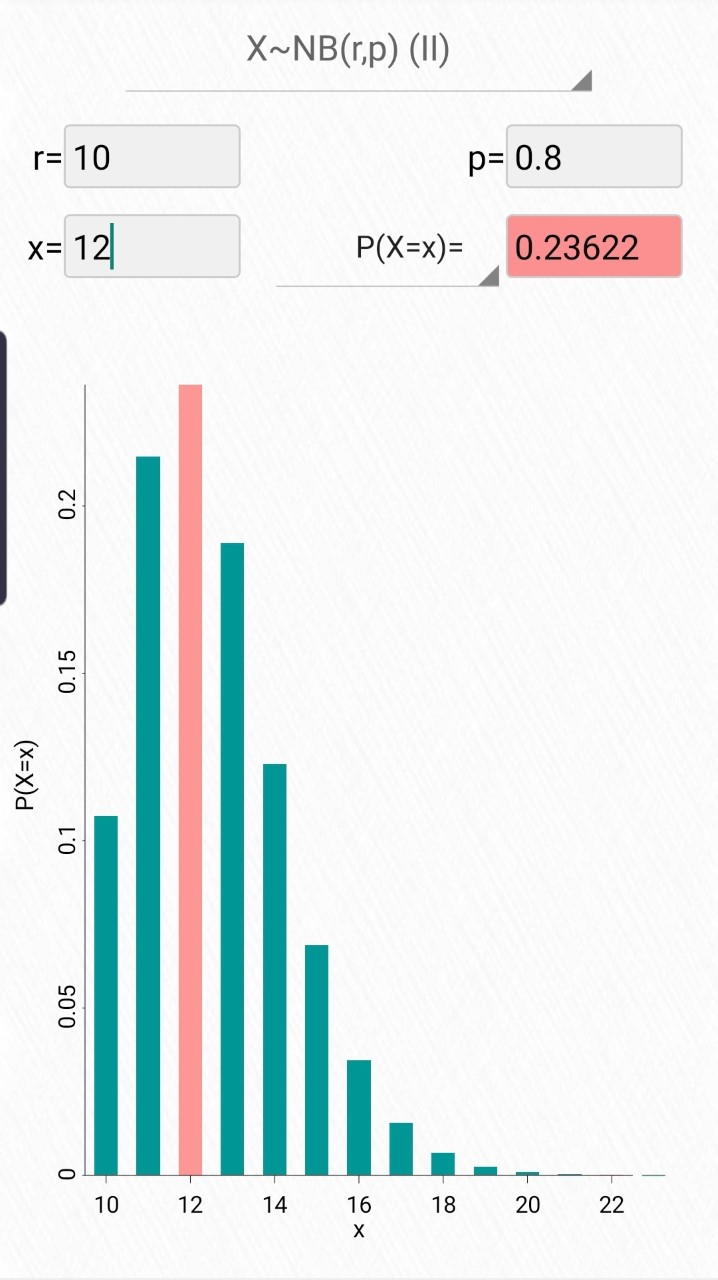
\includegraphics[width=0.4\linewidth]{IV.jpg}
		\end{figure}
	\end{frame}
	\begin{frame}{Ejemplo V}
	    \begin{examples}
    	    La probabilidad de que un bebe concebido sea niño es de 0,4, ¿En promedio cuantos hijos en total tendrá una pareja que desea tener tres niñas? Si x es el numero de niños antes de la tercera niña.
	    \end{examples}
	\end{frame}
\end{document}